\skipnexttoc
\section{自己紹介}
\begin{frame}
	こんにちは、びしょ〜j

	\pause
	% \bgroup\LARGE
	\bgroup\Huge
	\vspace{1\zw}
	これから\alert{\ruby{25日分のアドベントカレンダー}{\large{}闇のゲーム}}を

	\structure{5分}で進めるので自己紹介なんて時間かけられない。
	\vspace{1\zw}
	\egroup

	今日は12/02ということで\structure{2日目}から
\end{frame}
\section{2日目}
\begin{frame}[fragile]
	\frametitle{MoonScriptとは?}
	\begin{columns}
		\column[t]{.7\hsize}
		\begin{itemize}
			\item \alert{AltLua}で、PythonとかCoffeeScriptっぽい
			\item \lstinline|with|とか\structure{リスト内包表記}とか構文が増えている
			\item \lstinline|class|もあり、本格的な\structure{OOP}もできそう
		\end{itemize}
		\column[t]{.3\hsize}
		\begin{figure}[h]
			\vspace{-2\zw}\hspace{-5\zw}
\includegraphics[width=\columnwidth]{img/sailormoonscript.png}
		\end{figure}
	\end{columns}
	% \pause
	\begin{columns}
		\tiny
		\column[t]<2->{.4\hsize}
		\begin{lstlisting}[numbers=none,language=MoonScript,title=MoonScript class]
class Foo
	new: (@bar) =>
	baz: => print "bar: #{@bar}"
		\end{lstlisting}
		\uncover<3->{\hfill{}\structure{\normalsize{}compile! $\Rightarrow$}}

		\uncover<4->{
			{\LARGE{}\alert{かっこいい!! 短い!!}}

			オンラインコンパイラなどもあり手軽に始められる。詳しくは公式\footnote[frame]<4->{\url{http://moonscript.org/}}をチェッキラッ
		}
		\column[t]<3->{.6\hsize}
		\begin{lstlisting}[numbers=none,language={[5.3]lua},title=generated Lua]
local Foo
do
  local _base_0 = {
    baz = function(self)
      return print("bar: " .. tostring(self.bar))
    end
  }
  _base_0.__index = _base_0
  local _class_0 = setmetatable({
    __init = function(self, bar)
      self.bar = bar
    end,
    __base = _base_0,
    __name = "Foo"
........
		\end{lstlisting}
	\end{columns}
\end{frame}
\section{3日目}
\begin{frame}[fragile]
	\frametitle{わ〜〜い12/03は冴草きいちゃんの誕生日だ!!!!!}
	\begin{columns}
	\scriptsize
		\column[b]{.39\hsize}
		\begin{lstlisting}[numbers=none,language=MoonScript]
require'luakatsu'
Aikatsu.Kii!
-- name    冴草 きい
-- actor   秋奈
-- birthday        12/03
-- blood_type      O
-- favorite_foods  ブレインサンダー
-- special_ablity  パソコン
-- favorite_brand  MAGICAL TOY
-- type    Pop
-- signature_songs マジカルタイム
-- sing    市倉 有菜
-- school  ドリーム・アカデミー
		\end{lstlisting}
		\column[b]<2->{.62\hsize}
		\begin{lstlisting}[numbers=none,language=MoonScript,title=\alert{Luakatsu v3 draft function}]
require'luakatsu'
-- `find_birthday` returns matched idol table
((x) -> x and x!) (Aikatsu.find_birthday"12/03")
-- name    冴草 きい
-- actor   秋奈
-- birthday        12/03
-- blood_type      O
-- ...
		\end{lstlisting}
	\end{columns}
おめでとう! 秋奈さんもガルパン劇場版おめでとうございます!!!!

\pause
!!Luakatsu v3も\alert{12/03リリース}予定!!
\end{frame}
\section{4日目}
\begin{frame}[fragile]
	\frametitle{リスト内包表記}
	\bgroup\scriptsize
	\begin{lstlisting}[numbers=none,language=MoonScript]
t1 = {i for i = 1, 5}
-- {1, 2, 3, 4, 5}
t2 = {i for i = 1, 10 when i % 2 == 0}
-- {2, 4, 6, 8, 10}
t3 = {k, v * 3 for k, v in pairs{x:1, y:2, z:3}}
-- {x:3, y:6, z:9}
	\end{lstlisting}
	\egroup

	\pause
	これを用いてテーブルのdeep-copyも簡単にできる。
	\bgroup\scriptsize
	\begin{lstlisting}[numbers=none,language=MoonScript]
dc = (t) ->
	{k, (type(v) == "table" and (dc v) or v) for k, v in pairs t}
t = x: 1, y: 2, z: 3
t_ = dc t
t_.m = 4
print t.m -- nil
print t_.m -- 4
	\end{lstlisting}
	\egroup

\end{frame}
\section{5日目}
\begin{frame}[fragile]
	\frametitle{REPLがある\footnote[frame]{\url{https://github.com/Nymphium/moor/}}}

	MoonScriptの作者leafo氏がちょろっとかいたREPL\footnote[frame]{\url{https://github.com/leafo/moonscript/wiki/Moonscriptrepl}}を改良したもの\footnote[frame]{\url{https://luarocks.org/modules/steved/mooni/}}を改良した。
	一部オートインデントや、inspectモジュール\footnote[frame]{\url{https://github.com/kikito/inspect.lua/}}など使い勝手がよくなっているよ!
	\tiny
	\begin{lstlisting}[numbers=none]
$ moor -h
Usage: moonr [options]

   -h         print this message
   -n         continue running REPL after "e" option completed
   -e STR     execute string as MoonScript code
   -l LIB     load library before run REPL
   -L LIB     execute `LIB = require"LIB"` before run REPL

$ moor
moor on MoonScript version 0.3.2 on Lua 5.3
> string.split_t = (dlm) =>
?   [p for p in (@\match"#{dlm}$" and @ or @ .. dlm)\gmatch "(.-)#{dlm}"]
?
> "渋谷凛,島村卯月,本田未央"\split_t ","
{ "渋谷凛", "島村卯月", "本田未央" }
	\end{lstlisting}
\end{frame}
\section{6日目}
\begin{frame}[fragile]
	\frametitle{Syntax Checker for MoonScript}

	みなさんは\alert{Vim}/\structure{Neovim}を使っている可能性が高いと思いますが、Syntastic\footnote[frame]{強力なシンタックスチェッカープラグイン。\url{https://github.com/scrooloose/syntastic/}}%
	にMoonScriptのシンタックスチェッカーを書いた\footnote[frame]{\url{http://github.com/nymphium/syntastic-moonscript/}}。

	$\bullet$しくみ

	\vspace{-2\zw}
	\begin{columns}
		\column[t]{.6\hsize}
			\uncover<2->{
				\bgroup\small
				\begin{enumerate}
					\item ソースをLuaにコンパイル
					\item Luacheck\footnote[frame]{\url{http://luacheck.readthedocs.org/}}を通す
					\item \lstinline|moonc -X src.moon|でソースと生成されたLuaの行、エラー行を照らし合わせる(ここアホっぽい)
				\end{enumerate}
				\egroup
			}
		\column[t]{.4\hsize}
		\vspace{-2\zw}
		\begin{figure}[h]
			\centering
			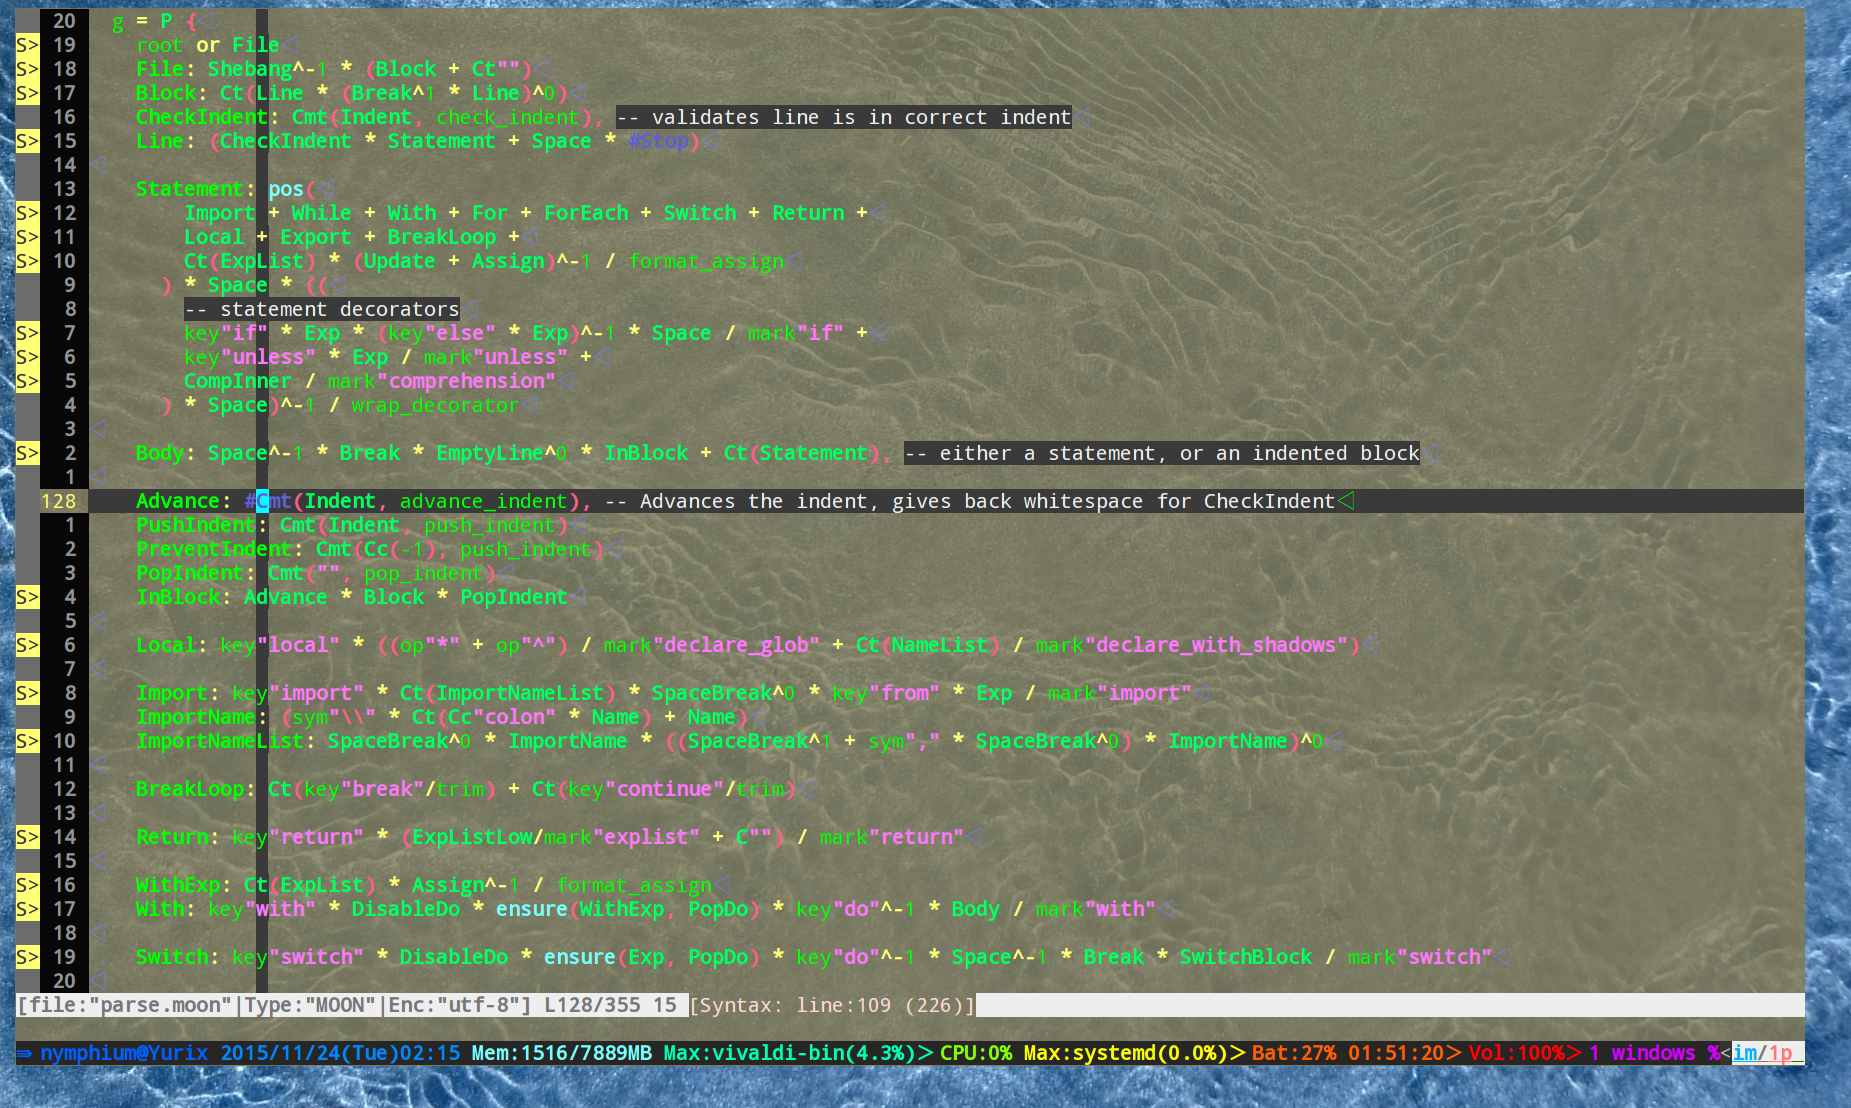
\includegraphics[width=\columnwidth]{img/syntastic.png}
		\end{figure}
	\end{columns}

	$\bullet$実装

	\begin{columns}
		\column[t]<3->{.2\hsize}
		\fbox{昔: シェルスクリプト}
		\column[t]<3->{.2\hsize}
		\vspace{-2\zw}
		\begin{center}
		$\Rightarrow$

		\uncover<5->{\alert{10倍速}
	
		{\tiny{}(もともとがしょぼかった)}}
		\end{center}
		\column[t]<4->{.2\hsize}
		\fbox{今: \structure{MoonScript}}
	\end{columns}
\end{frame}
